% Options for packages loaded elsewhere
\PassOptionsToPackage{unicode}{hyperref}
\PassOptionsToPackage{hyphens}{url}
%
\documentclass[
]{article}
\usepackage{amsmath,amssymb}
\usepackage{lmodern}
\usepackage{iftex}
\ifPDFTeX
  \usepackage[T1]{fontenc}
  \usepackage[utf8]{inputenc}
  \usepackage{textcomp} % provide euro and other symbols
\else % if luatex or xetex
  \usepackage{unicode-math}
  \defaultfontfeatures{Scale=MatchLowercase}
  \defaultfontfeatures[\rmfamily]{Ligatures=TeX,Scale=1}
\fi
% Use upquote if available, for straight quotes in verbatim environments
\IfFileExists{upquote.sty}{\usepackage{upquote}}{}
\IfFileExists{microtype.sty}{% use microtype if available
  \usepackage[]{microtype}
  \UseMicrotypeSet[protrusion]{basicmath} % disable protrusion for tt fonts
}{}
\makeatletter
\@ifundefined{KOMAClassName}{% if non-KOMA class
  \IfFileExists{parskip.sty}{%
    \usepackage{parskip}
  }{% else
    \setlength{\parindent}{0pt}
    \setlength{\parskip}{6pt plus 2pt minus 1pt}}
}{% if KOMA class
  \KOMAoptions{parskip=half}}
\makeatother
\usepackage{xcolor}
\usepackage[margin=1in]{geometry}
\usepackage{color}
\usepackage{fancyvrb}
\newcommand{\VerbBar}{|}
\newcommand{\VERB}{\Verb[commandchars=\\\{\}]}
\DefineVerbatimEnvironment{Highlighting}{Verbatim}{commandchars=\\\{\}}
% Add ',fontsize=\small' for more characters per line
\usepackage{framed}
\definecolor{shadecolor}{RGB}{248,248,248}
\newenvironment{Shaded}{\begin{snugshade}}{\end{snugshade}}
\newcommand{\AlertTok}[1]{\textcolor[rgb]{0.94,0.16,0.16}{#1}}
\newcommand{\AnnotationTok}[1]{\textcolor[rgb]{0.56,0.35,0.01}{\textbf{\textit{#1}}}}
\newcommand{\AttributeTok}[1]{\textcolor[rgb]{0.77,0.63,0.00}{#1}}
\newcommand{\BaseNTok}[1]{\textcolor[rgb]{0.00,0.00,0.81}{#1}}
\newcommand{\BuiltInTok}[1]{#1}
\newcommand{\CharTok}[1]{\textcolor[rgb]{0.31,0.60,0.02}{#1}}
\newcommand{\CommentTok}[1]{\textcolor[rgb]{0.56,0.35,0.01}{\textit{#1}}}
\newcommand{\CommentVarTok}[1]{\textcolor[rgb]{0.56,0.35,0.01}{\textbf{\textit{#1}}}}
\newcommand{\ConstantTok}[1]{\textcolor[rgb]{0.00,0.00,0.00}{#1}}
\newcommand{\ControlFlowTok}[1]{\textcolor[rgb]{0.13,0.29,0.53}{\textbf{#1}}}
\newcommand{\DataTypeTok}[1]{\textcolor[rgb]{0.13,0.29,0.53}{#1}}
\newcommand{\DecValTok}[1]{\textcolor[rgb]{0.00,0.00,0.81}{#1}}
\newcommand{\DocumentationTok}[1]{\textcolor[rgb]{0.56,0.35,0.01}{\textbf{\textit{#1}}}}
\newcommand{\ErrorTok}[1]{\textcolor[rgb]{0.64,0.00,0.00}{\textbf{#1}}}
\newcommand{\ExtensionTok}[1]{#1}
\newcommand{\FloatTok}[1]{\textcolor[rgb]{0.00,0.00,0.81}{#1}}
\newcommand{\FunctionTok}[1]{\textcolor[rgb]{0.00,0.00,0.00}{#1}}
\newcommand{\ImportTok}[1]{#1}
\newcommand{\InformationTok}[1]{\textcolor[rgb]{0.56,0.35,0.01}{\textbf{\textit{#1}}}}
\newcommand{\KeywordTok}[1]{\textcolor[rgb]{0.13,0.29,0.53}{\textbf{#1}}}
\newcommand{\NormalTok}[1]{#1}
\newcommand{\OperatorTok}[1]{\textcolor[rgb]{0.81,0.36,0.00}{\textbf{#1}}}
\newcommand{\OtherTok}[1]{\textcolor[rgb]{0.56,0.35,0.01}{#1}}
\newcommand{\PreprocessorTok}[1]{\textcolor[rgb]{0.56,0.35,0.01}{\textit{#1}}}
\newcommand{\RegionMarkerTok}[1]{#1}
\newcommand{\SpecialCharTok}[1]{\textcolor[rgb]{0.00,0.00,0.00}{#1}}
\newcommand{\SpecialStringTok}[1]{\textcolor[rgb]{0.31,0.60,0.02}{#1}}
\newcommand{\StringTok}[1]{\textcolor[rgb]{0.31,0.60,0.02}{#1}}
\newcommand{\VariableTok}[1]{\textcolor[rgb]{0.00,0.00,0.00}{#1}}
\newcommand{\VerbatimStringTok}[1]{\textcolor[rgb]{0.31,0.60,0.02}{#1}}
\newcommand{\WarningTok}[1]{\textcolor[rgb]{0.56,0.35,0.01}{\textbf{\textit{#1}}}}
\usepackage{graphicx}
\makeatletter
\def\maxwidth{\ifdim\Gin@nat@width>\linewidth\linewidth\else\Gin@nat@width\fi}
\def\maxheight{\ifdim\Gin@nat@height>\textheight\textheight\else\Gin@nat@height\fi}
\makeatother
% Scale images if necessary, so that they will not overflow the page
% margins by default, and it is still possible to overwrite the defaults
% using explicit options in \includegraphics[width, height, ...]{}
\setkeys{Gin}{width=\maxwidth,height=\maxheight,keepaspectratio}
% Set default figure placement to htbp
\makeatletter
\def\fps@figure{htbp}
\makeatother
\setlength{\emergencystretch}{3em} % prevent overfull lines
\providecommand{\tightlist}{%
  \setlength{\itemsep}{0pt}\setlength{\parskip}{0pt}}
\setcounter{secnumdepth}{-\maxdimen} % remove section numbering
\ifLuaTeX
  \usepackage{selnolig}  % disable illegal ligatures
\fi
\IfFileExists{bookmark.sty}{\usepackage{bookmark}}{\usepackage{hyperref}}
\IfFileExists{xurl.sty}{\usepackage{xurl}}{} % add URL line breaks if available
\urlstyle{same} % disable monospaced font for URLs
\hypersetup{
  pdftitle={Pensions ESG Pilot},
  pdfauthor={OVD},
  hidelinks,
  pdfcreator={LaTeX via pandoc}}

\title{Pensions ESG Pilot}
\author{OVD}
\date{2023-03-16}

\begin{document}
\maketitle

\begin{Shaded}
\begin{Highlighting}[]
\FunctionTok{setwd}\NormalTok{(}\AttributeTok{dir =} \StringTok{"/Users/ovd/Documents/GitHub/esg\_pensions"}\NormalTok{)}

\FunctionTok{options}\NormalTok{(}\AttributeTok{scipen=}\DecValTok{999}\NormalTok{)}
\end{Highlighting}
\end{Shaded}

\begin{Shaded}
\begin{Highlighting}[]
\FunctionTok{library}\NormalTok{(readr)}

\NormalTok{dfcj }\OtherTok{\textless{}{-}} \FunctionTok{read\_csv}\NormalTok{(}\StringTok{"rds\_prod.experiment.392385.stacked.csv"}\NormalTok{)}
\end{Highlighting}
\end{Shaded}

\begin{verbatim}
## Rows: 5664 Columns: 77
## -- Column specification --------------------------------------------------------
## Delimiter: ","
## chr  (20): EXPECTED_PENSION, INVESTS_IN_FIREARMS, INVESTS_IN_FOSSIL_FUELS, I...
## dbl  (55): RESPONDENT_ID, SURVEY_ID, CHOICE_SET, LABEL, CHOICE_INDICATOR, RE...
## dttm  (2): RESPONDENT_TIME_OF_OPENING_SURVEY, RESPONDENT_TIME_OF_COMPLETING_...
## 
## i Use `spec()` to retrieve the full column specification for this data.
## i Specify the column types or set `show_col_types = FALSE` to quiet this message.
\end{verbatim}

\begin{Shaded}
\begin{Highlighting}[]
\FunctionTok{library}\NormalTok{(cregg)}
\FunctionTok{library}\NormalTok{(janitor)}
\end{Highlighting}
\end{Shaded}

\begin{verbatim}
## 
## Attaching package: 'janitor'
\end{verbatim}

\begin{verbatim}
## The following objects are masked from 'package:stats':
## 
##     chisq.test, fisher.test
\end{verbatim}

\begin{Shaded}
\begin{Highlighting}[]
\FunctionTok{library}\NormalTok{(tidyverse)}
\end{Highlighting}
\end{Shaded}

\begin{verbatim}
## -- Attaching core tidyverse packages ------------------------ tidyverse 2.0.0 --
## v dplyr     1.1.0     v purrr     1.0.1
## v forcats   1.0.0     v stringr   1.5.0
## v ggplot2   3.4.1     v tibble    3.2.0
## v lubridate 1.9.2     v tidyr     1.3.0
\end{verbatim}

\begin{verbatim}
## -- Conflicts ------------------------------------------ tidyverse_conflicts() --
## x dplyr::filter() masks stats::filter()
## x dplyr::lag()    masks stats::lag()
## i Use the ]8;;http://conflicted.r-lib.org/conflicted package]8;; to force all conflicts to become errors
\end{verbatim}

\begin{Shaded}
\begin{Highlighting}[]
\FunctionTok{names}\NormalTok{(dfcj)}
\end{Highlighting}
\end{Shaded}

\begin{verbatim}
##  [1] "RESPONDENT_ID"                                                                                                               
##  [2] "SURVEY_ID"                                                                                                                   
##  [3] "CHOICE_SET"                                                                                                                  
##  [4] "LABEL"                                                                                                                       
##  [5] "CHOICE_INDICATOR"                                                                                                            
##  [6] "EXPECTED_PENSION"                                                                                                            
##  [7] "INVESTS_IN_FIREARMS"                                                                                                         
##  [8] "INVESTS_IN_FOSSIL_FUELS"                                                                                                     
##  [9] "INVESTS_IN_FIRMS_THAT_MAY_EMPLOY_CHILDREN"                                                                                   
## [10] "ADVOCATES_FOR_RACIAL_DIVERSITY_IN_MANAGEMENT"                                                                                
## [11] "ADVOCATES_FOR_EQUAL_PAY_FOR_MEN_AND_WOMEN"                                                                                   
## [12] "RESPONDENT_IP_ADDRESS"                                                                                                       
## [13] "RESPONDENT_CITY"                                                                                                             
## [14] "RESPONDENT_REGION"                                                                                                           
## [15] "RESPONDENT_POSTCODE"                                                                                                         
## [16] "RESPONDENT_COUNTRY"                                                                                                          
## [17] "RESPONDENT_TIME_OF_OPENING_SURVEY"                                                                                           
## [18] "RESPONDENT_TIME_OF_COMPLETING_SURVEY"                                                                                        
## [19] "RESPONDENT_DEVICE_USED_IN_SURVEY"                                                                                            
## [20] "RESPONDENT_LENGTH_OF_INTERVIEW_SECONDS"                                                                                      
## [21] "RESPONDENT_TOUCH_DEVICE_USED_IN_SURVEY"                                                                                      
## [22] "RESPONDENT_UNIQUE_CODE"                                                                                                      
## [23] "Q2_DO_YOU_CONSENT_TO_PARTICIPATING_IN_THIS_STUDY_O1_YES"                                                                     
## [24] "Q2_DO_YOU_CONSENT_TO_PARTICIPATING_IN_THIS_STUDY_O2_NO"                                                                      
## [25] "Q3_SCREEN_OUT"                                                                                                               
## [26] "Q5_WHAT_IS_THE_RESULT_OF_5_X_2_TO_MAKE_SURE_YOU_ARE_PAYING_ATTENTION_PLEASE_SELECT_THE_OPTION_NONE_OF_T_O1_10"               
## [27] "Q5_WHAT_IS_THE_RESULT_OF_5_X_2_TO_MAKE_SURE_YOU_ARE_PAYING_ATTENTION_PLEASE_SELECT_THE_OPTION_NONE_OF_T_O2_7"                
## [28] "Q5_WHAT_IS_THE_RESULT_OF_5_X_2_TO_MAKE_SURE_YOU_ARE_PAYING_ATTENTION_PLEASE_SELECT_THE_OPTION_NONE_OF_T_O3_12"               
## [29] "Q5_WHAT_IS_THE_RESULT_OF_5_X_2_TO_MAKE_SURE_YOU_ARE_PAYING_ATTENTION_PLEASE_SELECT_THE_OPTION_NONE_OF_T_O4_5"                
## [30] "Q5_WHAT_IS_THE_RESULT_OF_5_X_2_TO_MAKE_SURE_YOU_ARE_PAYING_ATTENTION_PLEASE_SELECT_THE_OPTION_NONE_OF_T_O5_8"                
## [31] "Q5_WHAT_IS_THE_RESULT_OF_5_X_2_TO_MAKE_SURE_YOU_ARE_PAYING_ATTENTION_PLEASE_SELECT_THE_OPTION_NONE_OF_T_O6_NONE_OF_THE_ABOVE"
## [32] "Q6_SCREEN_OUT"                                                                                                               
## [33] "Q7_WHAT_OF_THE_FOLLOWING_WORDS_IS_AN_ANIMAL_O1_DOG"                                                                          
## [34] "Q7_WHAT_OF_THE_FOLLOWING_WORDS_IS_AN_ANIMAL_O2_MOUNTAIN"                                                                     
## [35] "Q7_WHAT_OF_THE_FOLLOWING_WORDS_IS_AN_ANIMAL_O3_LAKE"                                                                         
## [36] "Q7_WHAT_OF_THE_FOLLOWING_WORDS_IS_AN_ANIMAL_O4_TREE"                                                                         
## [37] "Q7_WHAT_OF_THE_FOLLOWING_WORDS_IS_AN_ANIMAL_O5_CAR"                                                                          
## [38] "Q7_WHAT_OF_THE_FOLLOWING_WORDS_IS_AN_ANIMAL_O6_CAKE"                                                                         
## [39] "Q7_WHAT_OF_THE_FOLLOWING_WORDS_IS_AN_ANIMAL_O7_CANDLE"                                                                       
## [40] "Q8_SCREEN_OUT"                                                                                                               
## [41] "Q9_WOULD_YOU_PREFER_TO_RESTRICT_YOUR_INVESTMENTS_TO_FUNDS_THAT_TAKE_ENVIRONMENTAL_SOCIAL_AND_GOVERNANCE_O1_YES"              
## [42] "Q9_WOULD_YOU_PREFER_TO_RESTRICT_YOUR_INVESTMENTS_TO_FUNDS_THAT_TAKE_ENVIRONMENTAL_SOCIAL_AND_GOVERNANCE_O2_NO"               
## [43] "Q10_IN_WHAT_YEAR_WERE_YOU_BORN"                                                                                              
## [44] "Q11_WHAT_PARTY_DO_YOU_IDENTIFY_YOURSELF_WITH_O1_REPUBLICAN"                                                                  
## [45] "Q11_WHAT_PARTY_DO_YOU_IDENTIFY_YOURSELF_WITH_O2_DEMOCRAT"                                                                    
## [46] "Q11_WHAT_PARTY_DO_YOU_IDENTIFY_YOURSELF_WITH_O3_NONE"                                                                        
## [47] "Q12_IF_YOU_DON_T_IDENTIFY_WITH_ANY_PARTY_DO_YOU_LEAN_TOWARDS_ONE_OF_THEM_O1_REPUBLICAN"                                      
## [48] "Q12_IF_YOU_DON_T_IDENTIFY_WITH_ANY_PARTY_DO_YOU_LEAN_TOWARDS_ONE_OF_THEM_O2_DEMOCRAT"                                        
## [49] "Q12_IF_YOU_DON_T_IDENTIFY_WITH_ANY_PARTY_DO_YOU_LEAN_TOWARDS_ONE_OF_THEM_O3_NONE"                                            
## [50] "Q13_WHAT_GENDER_DO_YOU_IDENTIFY_WITH_O1_MALE"                                                                                
## [51] "Q13_WHAT_GENDER_DO_YOU_IDENTIFY_WITH_O2_FEMALE"                                                                              
## [52] "Q13_WHAT_GENDER_DO_YOU_IDENTIFY_WITH_O3_OTHER"                                                                               
## [53] "Q14_WHAT_ETHNICITY_DO_YOU_IDENTIFY_WITH_O1_WHITE"                                                                            
## [54] "Q14_WHAT_ETHNICITY_DO_YOU_IDENTIFY_WITH_O2_ASIAN"                                                                            
## [55] "Q14_WHAT_ETHNICITY_DO_YOU_IDENTIFY_WITH_O3_HISPANIC"                                                                         
## [56] "Q14_WHAT_ETHNICITY_DO_YOU_IDENTIFY_WITH_O4_AFRICAN_AMERICAN"                                                                 
## [57] "Q14_WHAT_ETHNICITY_DO_YOU_IDENTIFY_WITH_O5_NATIVE_AMERICAN"                                                                  
## [58] "Q14_WHAT_ETHNICITY_DO_YOU_IDENTIFY_WITH_O6_OTHER"                                                                            
## [59] "Q15_IN_WHAT_US_STATE_DO_YOU_LIVE_O1_FLORIDA"                                                                                 
## [60] "Q15_IN_WHAT_US_STATE_DO_YOU_LIVE_O2_TEXAS"                                                                                   
## [61] "Q15_IN_WHAT_US_STATE_DO_YOU_LIVE_O3_CALIFORNIA"                                                                              
## [62] "Q15_IN_WHAT_US_STATE_DO_YOU_LIVE_O4_NEW_YORK"                                                                                
## [63] "Q15_IN_WHAT_US_STATE_DO_YOU_LIVE_O5_OTHER"                                                                                   
## [64] "Q16_WHAT_IS_THE_HIGHEST_DEGREE_YOU_HAVE_EARNED_O1_SOME_HIGH_SCHOOL"                                                          
## [65] "Q16_WHAT_IS_THE_HIGHEST_DEGREE_YOU_HAVE_EARNED_O2_HIGH_SCHOOL"                                                               
## [66] "Q16_WHAT_IS_THE_HIGHEST_DEGREE_YOU_HAVE_EARNED_O3_SOME_COLLEGE"                                                              
## [67] "Q16_WHAT_IS_THE_HIGHEST_DEGREE_YOU_HAVE_EARNED_O4_COLLEGE_DEGREE"                                                            
## [68] "Q16_WHAT_IS_THE_HIGHEST_DEGREE_YOU_HAVE_EARNED_O5_GRADUATE_DEGREE"                                                           
## [69] "Q17_WHAT_IS_YOUR_GROSS_BEFORE_TAX_ANNUAL_INCOME"                                                                             
## [70] "Q18_HOW_MANY_DAYS_A_WEEK_DO_YOU_PRAY_OR_MEDITATE_O1_0"                                                                       
## [71] "Q18_HOW_MANY_DAYS_A_WEEK_DO_YOU_PRAY_OR_MEDITATE_O2_1"                                                                       
## [72] "Q18_HOW_MANY_DAYS_A_WEEK_DO_YOU_PRAY_OR_MEDITATE_O3_2"                                                                       
## [73] "Q18_HOW_MANY_DAYS_A_WEEK_DO_YOU_PRAY_OR_MEDITATE_O4_3"                                                                       
## [74] "Q18_HOW_MANY_DAYS_A_WEEK_DO_YOU_PRAY_OR_MEDITATE_O5_4"                                                                       
## [75] "Q18_HOW_MANY_DAYS_A_WEEK_DO_YOU_PRAY_OR_MEDITATE_O6_5"                                                                       
## [76] "Q18_HOW_MANY_DAYS_A_WEEK_DO_YOU_PRAY_OR_MEDITATE_O7_6"                                                                       
## [77] "Q18_HOW_MANY_DAYS_A_WEEK_DO_YOU_PRAY_OR_MEDITATE_O8_7"
\end{verbatim}

\begin{Shaded}
\begin{Highlighting}[]
\NormalTok{dfcj }\OtherTok{=}\NormalTok{ dfcj }\SpecialCharTok{\%\textgreater{}\%} 
  \FunctionTok{clean\_names}\NormalTok{() }

\NormalTok{dfcj }\SpecialCharTok{\%\textgreater{}\%} 
  \FunctionTok{filter}\NormalTok{(q3\_screen\_out }\SpecialCharTok{==} \StringTok{"NULL"} \SpecialCharTok{\&}\NormalTok{ q6\_screen\_out }\SpecialCharTok{==} \StringTok{"NULL"} \SpecialCharTok{\&}\NormalTok{ q8\_screen\_out }\SpecialCharTok{==} \StringTok{"NULL"}\NormalTok{) }\CommentTok{\# filter screen{-}outs (zero)}
\end{Highlighting}
\end{Shaded}

\begin{verbatim}
## # A tibble: 5,664 x 77
##    respo~1 surve~2 choic~3 label choic~4 expec~5 inves~6 inves~7 inves~8 advoc~9
##      <dbl>   <dbl>   <dbl> <dbl>   <dbl> <chr>   <chr>   <chr>   <chr>   <chr>  
##  1  1.83e8  1.83e8       1     1       0 Expect~ Invest~ Invest~ Invest~ Does n~
##  2  1.83e8  1.83e8       1     2       1 Expect~ Does n~ Does n~ Invest~ Advoca~
##  3  1.83e8  1.83e8       2     1       1 Expect~ Does n~ Does n~ Invest~ Advoca~
##  4  1.83e8  1.83e8       2     2       0 Expect~ Invest~ Invest~ Invest~ Does n~
##  5  1.83e8  1.83e8       3     1       0 Expect~ Does n~ Invest~ Invest~ Does n~
##  6  1.83e8  1.83e8       3     2       1 Expect~ Invest~ Does n~ Invest~ Advoca~
##  7  1.83e8  1.83e8       4     1       1 Expect~ Does n~ Does n~ Invest~ Does n~
##  8  1.83e8  1.83e8       4     2       0 Expect~ Invest~ Invest~ Invest~ Advoca~
##  9  1.83e8  1.83e8       5     1       0 Expect~ Invest~ Does n~ Invest~ Does n~
## 10  1.83e8  1.83e8       5     2       1 Expect~ Does n~ Invest~ Invest~ Advoca~
## # ... with 5,654 more rows, 67 more variables:
## #   advocates_for_equal_pay_for_men_and_women <chr>,
## #   respondent_ip_address <chr>, respondent_city <chr>,
## #   respondent_region <chr>, respondent_postcode <chr>,
## #   respondent_country <chr>, respondent_time_of_opening_survey <dttm>,
## #   respondent_time_of_completing_survey <dttm>,
## #   respondent_device_used_in_survey <chr>, ...
\end{verbatim}

\begin{Shaded}
\begin{Highlighting}[]
\NormalTok{median\_complet\_t }\OtherTok{=} \FunctionTok{median}\NormalTok{(dfcj}\SpecialCharTok{$}\NormalTok{respondent\_length\_of\_interview\_seconds) }\CommentTok{\# calculate median completion time in secs}

\NormalTok{ dfcj }\OtherTok{=}\NormalTok{ dfcj }\SpecialCharTok{\%\textgreater{}\%} 
  \FunctionTok{filter}\NormalTok{(respondent\_length\_of\_interview\_seconds }\SpecialCharTok{\textgreater{}=} \FloatTok{0.5} \SpecialCharTok{*}\NormalTok{ median\_complet\_t,}
\NormalTok{         respondent\_length\_of\_interview\_seconds }\SpecialCharTok{\textless{}=} \FloatTok{1.5} \SpecialCharTok{*}\NormalTok{ median\_complet\_t) }\CommentTok{\# filter responded too quickly or slowly}

\FunctionTok{table}\NormalTok{(dfcj}\SpecialCharTok{$}\NormalTok{invests\_in\_firearms)}
\end{Highlighting}
\end{Shaded}

\begin{verbatim}
## 
## Does not invest in firearms         Invests in firearms 
##                        2510                        2506
\end{verbatim}

\begin{Shaded}
\begin{Highlighting}[]
\FunctionTok{table}\NormalTok{(dfcj}\SpecialCharTok{$}\NormalTok{invests\_in\_firms\_that\_may\_employ\_children)}
\end{Highlighting}
\end{Shaded}

\begin{verbatim}
## 
## Invests in firms that ensure no children are employed 
##                                                  2513 
##             Invests in firms that may employ children 
##                                                  2503
\end{verbatim}

\begin{Shaded}
\begin{Highlighting}[]
\FunctionTok{table}\NormalTok{(dfcj}\SpecialCharTok{$}\NormalTok{advocates\_for\_racial\_diversity\_in\_management)}
\end{Highlighting}
\end{Shaded}

\begin{verbatim}
## 
##         Advocates for racial diversity in management 
##                                                 2506 
## Does not advocate for racial diversity in management 
##                                                 2510
\end{verbatim}

\begin{Shaded}
\begin{Highlighting}[]
\CommentTok{\# create vars for AMCE}

\FunctionTok{typeof}\NormalTok{(dfcj}\SpecialCharTok{$}\NormalTok{expected\_pension)}
\end{Highlighting}
\end{Shaded}

\begin{verbatim}
## [1] "character"
\end{verbatim}

\begin{Shaded}
\begin{Highlighting}[]
\CommentTok{\# levels(dfcj1$expected\_pension\_num) = c("$20,000", "$25,000", "$30,000", "$35,000", "$40,000", "$45,000", "$50,000")}

\NormalTok{dfcj1 }\OtherTok{=}\NormalTok{ dfcj }\SpecialCharTok{\%\textgreater{}\%} 
  \FunctionTok{mutate}\NormalTok{(}\AttributeTok{expected\_pension\_num =} \FunctionTok{factor}\NormalTok{(expected\_pension),}
         \AttributeTok{firearms =} \FunctionTok{factor}\NormalTok{(invests\_in\_firearms),}
         \AttributeTok{fossil\_fuels =}  \FunctionTok{factor}\NormalTok{(invests\_in\_fossil\_fuels),}
         \AttributeTok{may\_employ\_children =} \FunctionTok{factor}\NormalTok{(invests\_in\_firms\_that\_may\_employ\_children),}
         \AttributeTok{racial\_diversity =} \FunctionTok{factor}\NormalTok{(advocates\_for\_racial\_diversity\_in\_management),}
         \AttributeTok{gender\_equal\_pay =} \FunctionTok{factor}\NormalTok{(advocates\_for\_equal\_pay\_for\_men\_and\_women))}
                                   

\NormalTok{dfcj7 }\OtherTok{=}\NormalTok{ dfcj }\SpecialCharTok{\%\textgreater{}\%}
  \FunctionTok{mutate}\NormalTok{(}\AttributeTok{expected\_pension\_num =} \FunctionTok{factor}\NormalTok{(expected\_pension,}
                                       \AttributeTok{levels =} \FunctionTok{c}\NormalTok{(}\StringTok{"$20,000"}\NormalTok{, }\StringTok{"$25,000"}\NormalTok{, }\StringTok{"$30,000"}\NormalTok{, }\StringTok{"$35,000"}\NormalTok{, }\StringTok{"$40,000"}\NormalTok{, }\StringTok{"$45,000"}\NormalTok{, }\StringTok{"$50,000"}\NormalTok{)),}
         \AttributeTok{firearms =} \FunctionTok{factor}\NormalTok{(invests\_in\_firearms,}
                           \AttributeTok{levels =} \FunctionTok{c}\NormalTok{(}\StringTok{"yes"}\NormalTok{, }\StringTok{"no"}\NormalTok{)),}
         \AttributeTok{fossil\_fuels =}  \FunctionTok{factor}\NormalTok{(invests\_in\_fossil\_fuels,}
                                \AttributeTok{levels =} \FunctionTok{c}\NormalTok{(}\StringTok{"yes"}\NormalTok{, }\StringTok{"no"}\NormalTok{)),}
         \AttributeTok{may\_employ\_children =} \FunctionTok{factor}\NormalTok{(invests\_in\_firms\_that\_may\_employ\_children,}
                                      \AttributeTok{levels =} \FunctionTok{c}\NormalTok{(}\StringTok{"yes"}\NormalTok{, }\StringTok{"no"}\NormalTok{)),}
         \AttributeTok{racial\_diversity =} \FunctionTok{factor}\NormalTok{(advocates\_for\_racial\_diversity\_in\_management,}
                                   \AttributeTok{levels =} \FunctionTok{c}\NormalTok{(}\StringTok{"no"}\NormalTok{, }\StringTok{"yes"}\NormalTok{)),}
         \AttributeTok{gender\_equal\_pay =} \FunctionTok{factor}\NormalTok{(advocates\_for\_equal\_pay\_for\_men\_and\_women,}
                                   \AttributeTok{levels =} \FunctionTok{c}\NormalTok{(}\StringTok{"no"}\NormalTok{, }\StringTok{"yes"}\NormalTok{)))}
\end{Highlighting}
\end{Shaded}

\begin{Shaded}
\begin{Highlighting}[]
\CommentTok{\# Something went wrong here}
\CommentTok{\# }
\CommentTok{\# labels(dfcj1$expected\_pension\_num) \textless{}{-} list("$20,000" = "Expected pension: $20,000 a year", }
\CommentTok{\#                                         "$25,000" = "Expected pension: $25,000 a year", }
\CommentTok{\#                                         "30,000"= "Expected pension: $30,000 a year", }
\CommentTok{\#                                        "$35,000" = "Expected pension: $35,000 a year", }
\CommentTok{\#                                         "$40,000" = "Expected pension: $40,000 a year", }
\CommentTok{\#                                         "$45,000" = "Expected pension: $45,000 a year", }
\CommentTok{\#                                          "$50,000" = "Expected pension: $50,000 a year")}
\CommentTok{\# }
\CommentTok{\# labels(dfcj1$firearms) \textless{}{-} list("yes" = "Invests in firearms",}
\CommentTok{\#                                "no" = "Does not invest in firearms")}
\CommentTok{\# }
\CommentTok{\# labels(dfcj1$fossil\_fuels) \textless{}{-} list("yes" = "Invests in fossil fuels",}
\CommentTok{\#                                 "no" = "Does not invest in fossil fuels")}
\CommentTok{\# }
\CommentTok{\# labels(dfcj1$may\_employ\_children) \textless{}{-} list("yes" = "Invests in firms that may employ children",}
\CommentTok{\#                                        "no" = "Invests in firms that ensure no children are employed")}
\CommentTok{\# }
\CommentTok{\# labels(dfcj1$racial\_diversity) \textless{}{-} list("yes" = "Advocates for racial diversity in management",}
\CommentTok{\#                                     "no" = "Does not advocate for racial diversity in management")}
\CommentTok{\# }
\CommentTok{\# labels(dfcj1$gender\_equal\_pay) \textless{}{-} list("yes" = "Advocates for equal pay for men and women",}
\CommentTok{\#                                     "no" = "Does not advocate for equal pay for men and women")}
\end{Highlighting}
\end{Shaded}

Try with case\_when instead

\begin{Shaded}
\begin{Highlighting}[]
\NormalTok{dfcj7 }\OtherTok{=}\NormalTok{ dfcj }\SpecialCharTok{\%\textgreater{}\%}
  \FunctionTok{mutate}\NormalTok{(}\AttributeTok{expected\_pension\_num =} \FunctionTok{factor}\NormalTok{(expected\_pension),}
         \AttributeTok{firearms =} \FunctionTok{factor}\NormalTok{(invests\_in\_firearms),                           }
         \AttributeTok{fossil\_fuels =}  \FunctionTok{factor}\NormalTok{(invests\_in\_fossil\_fuels),}
         \AttributeTok{may\_employ\_children =} \FunctionTok{factor}\NormalTok{(invests\_in\_firms\_that\_may\_employ\_children),}
         \AttributeTok{racial\_diversity =} \FunctionTok{factor}\NormalTok{(advocates\_for\_racial\_diversity\_in\_management),}
        \AttributeTok{gender\_equal\_pay =} \FunctionTok{factor}\NormalTok{(advocates\_for\_equal\_pay\_for\_men\_and\_women))}


\NormalTok{dfcj7}\SpecialCharTok{$}\NormalTok{expected\_pension\_num }\OtherTok{\textless{}{-}} \FunctionTok{recode}\NormalTok{(dfcj7}\SpecialCharTok{$}\NormalTok{expected\_pension\_num,}
                                     \StringTok{"Expected pension: $20,000 a year"} \OtherTok{=} \StringTok{"20000"}\NormalTok{, }
                                        \StringTok{"Expected pension: $25,000 a year"} \OtherTok{=} \StringTok{"25000"}\NormalTok{, }
                                        \StringTok{"Expected pension: $30,000 a year"} \OtherTok{=} \StringTok{"30000"}\NormalTok{, }
                                       \StringTok{"Expected pension: $35,000 a year"} \OtherTok{=} \StringTok{"35000"}\NormalTok{, }
                                        \StringTok{"Expected pension: $40,000 a year"} \OtherTok{=} \StringTok{"40000"}\NormalTok{, }
                                        \StringTok{"Expected pension: $45,000 a year"} \OtherTok{=} \StringTok{"45000"}\NormalTok{, }
                                        \StringTok{"Expected pension: $50,000 a year"} \OtherTok{=} \StringTok{"50000"}\NormalTok{)}

\NormalTok{dfcj7}\SpecialCharTok{$}\NormalTok{firearms }\OtherTok{\textless{}{-}} \FunctionTok{recode}\NormalTok{(dfcj7}\SpecialCharTok{$}\NormalTok{firearms,}
                         \StringTok{"Invests in firearms"} \OtherTok{=} \StringTok{"yes"}\NormalTok{,}
                         \StringTok{"Does not invest in firearms"} \OtherTok{=} \StringTok{"no"}\NormalTok{)}

\NormalTok{dfcj7}\SpecialCharTok{$}\NormalTok{fossil\_fuels }\OtherTok{\textless{}{-}} \FunctionTok{recode}\NormalTok{(dfcj7}\SpecialCharTok{$}\NormalTok{fossil\_fuels,}
                             \StringTok{"Invests in fossil fuels"} \OtherTok{=} \StringTok{"yes"}\NormalTok{,}
                              \StringTok{"Does not invest in fossil fuels"} \OtherTok{=} \StringTok{"no"}\NormalTok{)}

\NormalTok{dfcj7}\SpecialCharTok{$}\NormalTok{may\_employ\_children }\OtherTok{\textless{}{-}} \FunctionTok{recode}\NormalTok{(dfcj7}\SpecialCharTok{$}\NormalTok{may\_employ\_children,}
                                    \StringTok{"Invests in firms that may employ children"} \OtherTok{=} \StringTok{"yes"}\NormalTok{,}
                                    \StringTok{"Invests in firms that ensure no children are employed"} \OtherTok{=} \StringTok{"no"}\NormalTok{)}

\NormalTok{dfcj7}\SpecialCharTok{$}\NormalTok{racial\_diversity }\OtherTok{\textless{}{-}} \FunctionTok{recode}\NormalTok{(dfcj7}\SpecialCharTok{$}\NormalTok{racial\_diversity,}
                                \StringTok{"Advocates for racial diversity in management"} \OtherTok{=} \StringTok{"yes"}\NormalTok{,}
                                \StringTok{"Does not advocate for racial diversity in management"} \OtherTok{=} \StringTok{"no"}\NormalTok{)}

\NormalTok{dfcj7}\SpecialCharTok{$}\NormalTok{gender\_equal\_pay }\OtherTok{\textless{}{-}} \FunctionTok{recode}\NormalTok{(dfcj7}\SpecialCharTok{$}\NormalTok{gender\_equal\_pay,}
                                 \StringTok{"Advocates for equal pay for men and women"} \OtherTok{=} \StringTok{"yes"}\NormalTok{,}
                                 \StringTok{"Does not advocate for equal pay for men and women"} \OtherTok{=} \StringTok{"no"}\NormalTok{)}
\end{Highlighting}
\end{Shaded}

\begin{Shaded}
\begin{Highlighting}[]
\NormalTok{dfcj1}\SpecialCharTok{$}\NormalTok{expected\_pension\_num }\OtherTok{\textless{}{-}} \FunctionTok{recode}\NormalTok{(dfcj1}\SpecialCharTok{$}\NormalTok{expected\_pension\_num,}
                                     \StringTok{"Expected pension: $20,000 a year"} \OtherTok{=} \StringTok{"20000"}\NormalTok{, }
                                        \StringTok{"Expected pension: $25,000 a year"} \OtherTok{=} \StringTok{"25000"}\NormalTok{, }
                                        \StringTok{"Expected pension: $30,000 a year"} \OtherTok{=} \StringTok{"30000"}\NormalTok{, }
                                       \StringTok{"Expected pension: $35,000 a year"} \OtherTok{=} \StringTok{"35000"}\NormalTok{, }
                                        \StringTok{"Expected pension: $40,000 a year"} \OtherTok{=} \StringTok{"40000"}\NormalTok{, }
                                        \StringTok{"Expected pension: $45,000 a year"} \OtherTok{=} \StringTok{"45000"}\NormalTok{, }
                                        \StringTok{"Expected pension: $50,000 a year"} \OtherTok{=} \StringTok{"50000"}\NormalTok{)}


\NormalTok{dfcj1}\SpecialCharTok{$}\NormalTok{firearms }\OtherTok{\textless{}{-}} \FunctionTok{recode}\NormalTok{(dfcj1}\SpecialCharTok{$}\NormalTok{firearms,}
                         \StringTok{"Invests in firearms"} \OtherTok{=} \StringTok{"yes"}\NormalTok{,}
                         \StringTok{"Does not invest in firearms"} \OtherTok{=} \StringTok{"no"}\NormalTok{)}

\NormalTok{dfcj1}\SpecialCharTok{$}\NormalTok{fossil\_fuels }\OtherTok{\textless{}{-}} \FunctionTok{recode}\NormalTok{(dfcj1}\SpecialCharTok{$}\NormalTok{fossil\_fuels,}
                             \StringTok{"Invests in fossil fuels"} \OtherTok{=} \StringTok{"yes"}\NormalTok{,}
                              \StringTok{"Does not invest in fossil fuels"} \OtherTok{=} \StringTok{"no"}\NormalTok{)}

\NormalTok{dfcj1}\SpecialCharTok{$}\NormalTok{may\_employ\_children }\OtherTok{\textless{}{-}} \FunctionTok{recode}\NormalTok{(dfcj1}\SpecialCharTok{$}\NormalTok{may\_employ\_children,}
                                    \StringTok{"Invests in firms that may employ children"} \OtherTok{=} \StringTok{"yes"}\NormalTok{,}
                                    \StringTok{"Invests in firms that ensure no children are employed"} \OtherTok{=} \StringTok{"no"}\NormalTok{)}

\NormalTok{dfcj1}\SpecialCharTok{$}\NormalTok{racial\_diversity }\OtherTok{\textless{}{-}} \FunctionTok{recode}\NormalTok{(dfcj1}\SpecialCharTok{$}\NormalTok{racial\_diversity,}
                                \StringTok{"Advocates for racial diversity in management"} \OtherTok{=} \StringTok{"yes"}\NormalTok{,}
                                \StringTok{"Does not advocate for racial diversity in management"} \OtherTok{=} \StringTok{"no"}\NormalTok{)}

\NormalTok{dfcj1}\SpecialCharTok{$}\NormalTok{gender\_equal\_pay }\OtherTok{\textless{}{-}} \FunctionTok{recode}\NormalTok{(dfcj1}\SpecialCharTok{$}\NormalTok{gender\_equal\_pay,}
                                 \StringTok{"Advocates for equal pay for men and women"} \OtherTok{=} \StringTok{"yes"}\NormalTok{,}
                                 \StringTok{"Does not advocate for equal pay for men and women"} \OtherTok{=} \StringTok{"no"}\NormalTok{)}
\end{Highlighting}
\end{Shaded}

\begin{Shaded}
\begin{Highlighting}[]
\CommentTok{\# change var type      }
\NormalTok{dfcj1 }\OtherTok{=}\NormalTok{ dfcj1 }\SpecialCharTok{\%\textgreater{}\%} 
  \FunctionTok{mutate}\NormalTok{(}\AttributeTok{choice\_indicator =} \FunctionTok{as.numeric}\NormalTok{(choice\_indicator)) }

\NormalTok{dfcj7 }\OtherTok{=}\NormalTok{ dfcj7 }\SpecialCharTok{\%\textgreater{}\%} 
  \FunctionTok{mutate}\NormalTok{(}\AttributeTok{choice\_indicator =} \FunctionTok{as.numeric}\NormalTok{(choice\_indicator)) }

\CommentTok{\#relevel factors}
\CommentTok{\# dfcj1$racial\_diversity \textless{}{-} relevel(dfcj1$racial\_diversity, "no")}
\CommentTok{\# }
\CommentTok{\# dfcj1$gender\_equal\_pay \textless{}{-} relevel(dfcj1$gender\_equal\_pay, "no")}
\end{Highlighting}
\end{Shaded}

\begin{Shaded}
\begin{Highlighting}[]
\CommentTok{\#check sample size}

\NormalTok{dfcj1 }\SpecialCharTok{\%\textgreater{}\%} 
  \FunctionTok{distinct}\NormalTok{(respondent\_id, }\AttributeTok{.keep\_all =}\NormalTok{ T) }\SpecialCharTok{\%\textgreater{}\%} 
  \FunctionTok{count}\NormalTok{()}
\end{Highlighting}
\end{Shaded}

\begin{verbatim}
## # A tibble: 1 x 1
##       n
##   <int>
## 1   209
\end{verbatim}

\begin{Shaded}
\begin{Highlighting}[]
\CommentTok{\#trying to debug}
\NormalTok{dfcj }\OtherTok{=}\NormalTok{ dfcj }\SpecialCharTok{\%\textgreater{}\%} 
  \FunctionTok{mutate}\NormalTok{(}\AttributeTok{expected\_pension\_num =} \FunctionTok{factor}\NormalTok{(expected\_pension),}
         \AttributeTok{firearms =} \FunctionTok{factor}\NormalTok{(invests\_in\_firearms),                              }
         \AttributeTok{fossil\_fuels =}  \FunctionTok{factor}\NormalTok{(invests\_in\_fossil\_fuels),}
         \AttributeTok{may\_employ\_children =} \FunctionTok{factor}\NormalTok{(invests\_in\_firms\_that\_may\_employ\_children), }
         \AttributeTok{racial\_diversity =} \FunctionTok{factor}\NormalTok{(advocates\_for\_racial\_diversity\_in\_management),}
         \AttributeTok{gender\_equal\_pay =} \FunctionTok{factor}\NormalTok{(advocates\_for\_equal\_pay\_for\_men\_and\_women),}
        \AttributeTok{choice\_indicator =} \FunctionTok{as.numeric}\NormalTok{(choice\_indicator))}

\CommentTok{\# This worked in AMCE. What did I do wrong when re{-}leveling the factors???}
\end{Highlighting}
\end{Shaded}

\begin{Shaded}
\begin{Highlighting}[]
\NormalTok{dfcj2 }\OtherTok{=}\NormalTok{ dfcj1 }\SpecialCharTok{\%\textgreater{}\%} 
  \FunctionTok{select}\NormalTok{(survey\_id, choice\_indicator, expected\_pension\_num, firearms, fossil\_fuels, may\_employ\_children, racial\_diversity, gender\_equal\_pay)}

\NormalTok{f1 }\OtherTok{\textless{}{-}}\NormalTok{ choice\_indicator }\SpecialCharTok{\textasciitilde{}}\NormalTok{ expected\_pension\_num }\SpecialCharTok{+}\NormalTok{ firearms }\SpecialCharTok{+}\NormalTok{ fossil\_fuels }\SpecialCharTok{+}\NormalTok{ may\_employ\_children }\SpecialCharTok{+}\NormalTok{ racial\_diversity }\SpecialCharTok{+}\NormalTok{ gender\_equal\_pay}

\CommentTok{\# This does not work because there is an issue with the factor levels. I should check this later}
\CommentTok{\#amce2 = amce(dfcj7, f1, id = \textasciitilde{} survey\_id)}
                        
\FunctionTok{table}\NormalTok{(dfcj1}\SpecialCharTok{$}\NormalTok{firearms)}
\end{Highlighting}
\end{Shaded}

\begin{verbatim}
## 
##   no  yes 
## 2510 2506
\end{verbatim}

\begin{Shaded}
\begin{Highlighting}[]
\CommentTok{\# plot(amce)}
\end{Highlighting}
\end{Shaded}

\begin{Shaded}
\begin{Highlighting}[]
\CommentTok{\#Did not work... wtf is going on with factors.... ask in github or stackexchange}

\NormalTok{dfcjlab }\OtherTok{=}\NormalTok{ dfcj }


\NormalTok{dfcjlab}\SpecialCharTok{$}\NormalTok{firearms  }\OtherTok{=} \FunctionTok{relevel}\NormalTok{(dfcjlab}\SpecialCharTok{$}\NormalTok{firearms, }\StringTok{"Invests in firearms"}\NormalTok{)}

\NormalTok{dfcjlab}\SpecialCharTok{$}\NormalTok{fossil\_fuels }\OtherTok{=} \FunctionTok{relevel}\NormalTok{(dfcjlab}\SpecialCharTok{$}\NormalTok{fossil\_fuels, }\StringTok{"Invests in fossil fuels"}\NormalTok{)}

\NormalTok{dfcjlab}\SpecialCharTok{$}\NormalTok{may\_employ\_children }\OtherTok{=} \FunctionTok{relevel}\NormalTok{(dfcjlab}\SpecialCharTok{$}\NormalTok{may\_employ\_children, }\StringTok{"Invests in firms that may employ children"}\NormalTok{)}

\NormalTok{dfcjlab}\SpecialCharTok{$}\NormalTok{racial\_diversity }\OtherTok{=} \FunctionTok{relevel}\NormalTok{(dfcjlab}\SpecialCharTok{$}\NormalTok{racial\_diversity, }\StringTok{"Does not advocate for racial diversity in management"}\NormalTok{)}

\NormalTok{dfcjlab}\SpecialCharTok{$}\NormalTok{gender\_equal\_pay }\OtherTok{=} \FunctionTok{relevel}\NormalTok{(dfcjlab}\SpecialCharTok{$}\NormalTok{gender\_equal\_pay, }\StringTok{"Does not advocate for equal pay for men and women"}\NormalTok{)}
\end{Highlighting}
\end{Shaded}

\begin{Shaded}
\begin{Highlighting}[]
\FunctionTok{levels}\NormalTok{(dfcj}\SpecialCharTok{$}\NormalTok{gender\_equal\_pay)}
\end{Highlighting}
\end{Shaded}

\begin{verbatim}
## [1] "Advocates for equal pay for men and women"        
## [2] "Does not advocate for equal pay for men and women"
\end{verbatim}

\begin{Shaded}
\begin{Highlighting}[]
\CommentTok{\#with factors re leveled}

\NormalTok{amce1 }\OtherTok{=} \FunctionTok{amce}\NormalTok{(dfcjlab, f1, }\AttributeTok{id =} \SpecialCharTok{\textasciitilde{}}\NormalTok{ survey\_id)}
\end{Highlighting}
\end{Shaded}

\begin{verbatim}
## Warning in logLik.svyglm(x): svyglm not fitted by maximum likelihood.
\end{verbatim}

\begin{Shaded}
\begin{Highlighting}[]
\FunctionTok{plot}\NormalTok{(amce1)}
\end{Highlighting}
\end{Shaded}

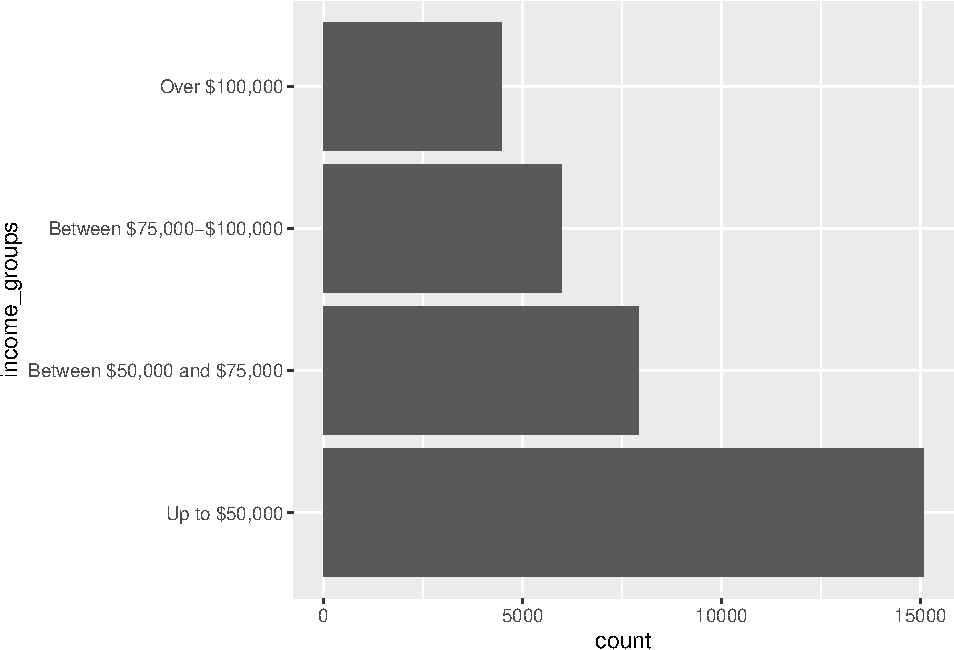
\includegraphics{analysis_march16_files/figure-latex/unnamed-chunk-16-1.pdf}

WTP analysis

\begin{Shaded}
\begin{Highlighting}[]
\FunctionTok{library}\NormalTok{(logitr)}
\end{Highlighting}
\end{Shaded}

\begin{verbatim}
## Version:  1.0.1
## Author:   John Paul Helveston (George Washington University)
## 
## Consider submitting praise at
## https://github.com/jhelvy/logitr/issues/8.
## 
## Please cite the JSS article in your publications, see:
## citation("logitr")
\end{verbatim}

\begin{Shaded}
\begin{Highlighting}[]
\NormalTok{dfcjtest }\OtherTok{=}\NormalTok{ dfcj }\SpecialCharTok{\%\textgreater{}\%} 
  \FunctionTok{mutate}\NormalTok{(}\AttributeTok{pension =}\NormalTok{ expected\_pension)}

\CommentTok{\# dfcjtest = dfcjtest \%\textgreater{}\% }
\CommentTok{\#   mutate(pension = factor(expected\_pension,}
\CommentTok{\#                           levels = c("20,000",}
\CommentTok{\#                                      "25,000",}
\CommentTok{\#                                      "30,000",}
\CommentTok{\#                                      "35,000",}
\CommentTok{\#                                      "40,000",}
\CommentTok{\#                                      "45,000",}
\CommentTok{\#                                      "50,000")))}

\NormalTok{dfcjtest}\SpecialCharTok{$}\NormalTok{pension }\OtherTok{\textless{}{-}} \FunctionTok{recode}\NormalTok{(dfcjtest}\SpecialCharTok{$}\NormalTok{pension,}
                                     \StringTok{"Expected pension: $20,000 a year"} \OtherTok{=} \StringTok{"20,000"}\NormalTok{, }
                                        \StringTok{"Expected pension: $25,000 a year"} \OtherTok{=} \StringTok{"25,000"}\NormalTok{, }
                                        \StringTok{"Expected pension: $30,000 a year"} \OtherTok{=} \StringTok{"30,000"}\NormalTok{, }
                                       \StringTok{"Expected pension: $35,000 a year"} \OtherTok{=} \StringTok{"35,000"}\NormalTok{, }
                                        \StringTok{"Expected pension: $40,000 a year"} \OtherTok{=} \StringTok{"40,000"}\NormalTok{, }
                                        \StringTok{"Expected pension: $45,000 a year"} \OtherTok{=} \StringTok{"45,000"}\NormalTok{, }
                                        \StringTok{"Expected pension: $50,000 a year"} \OtherTok{=} \StringTok{"50,000"}\NormalTok{)}
\end{Highlighting}
\end{Shaded}

\begin{Shaded}
\begin{Highlighting}[]
 \FunctionTok{table}\NormalTok{(dfcjtest}\SpecialCharTok{$}\NormalTok{pension) }
\end{Highlighting}
\end{Shaded}

\begin{verbatim}
## 
## 20,000 25,000 30,000 35,000 40,000 45,000 50,000 
##    716    725    715    711    713    720    716
\end{verbatim}

\begin{Shaded}
\begin{Highlighting}[]
\FunctionTok{typeof}\NormalTok{(dfcjtest}\SpecialCharTok{$}\NormalTok{pension)}
\end{Highlighting}
\end{Shaded}

\begin{verbatim}
## [1] "character"
\end{verbatim}

\begin{Shaded}
\begin{Highlighting}[]
\CommentTok{\# }
\CommentTok{\# }
\CommentTok{\# dfcjtest2 = dfcjtest \%\textgreater{}\%}
\CommentTok{\#   mutate(pension\_num2 = as.numeric(pension))}
\CommentTok{\# }
\CommentTok{\# table(dfcjtest2$pension\_num2)}
\CommentTok{\# }
\CommentTok{\# dfcjtest2$pension}
\CommentTok{\# }
\CommentTok{\# dfcjtest$pension\_num = as.numeric(dfcjtest$pension\_num)}

\CommentTok{\# ,}
\CommentTok{\#            id = as.integer(survey\_id))}

\NormalTok{dfcjtest }\OtherTok{=}\NormalTok{ dfcjtest }\SpecialCharTok{\%\textgreater{}\%}
   \FunctionTok{mutate}\NormalTok{(}\AttributeTok{pension\_num =}\NormalTok{ readr}\SpecialCharTok{::}\FunctionTok{parse\_number}\NormalTok{(pension)) }
\end{Highlighting}
\end{Shaded}

\begin{Shaded}
\begin{Highlighting}[]
\FunctionTok{library}\NormalTok{(readxl)}
\NormalTok{nochoice }\OtherTok{\textless{}{-}} \FunctionTok{read\_excel}\NormalTok{(}\StringTok{"\textasciitilde{}/Documents/GitHub/esg\_pensions/nochoice.xlsx"}\NormalTok{)}
\end{Highlighting}
\end{Shaded}

\begin{Shaded}
\begin{Highlighting}[]
\NormalTok{ncl }\OtherTok{=} \FunctionTok{pivot\_longer}\NormalTok{(nochoice, }\AttributeTok{cols =}\NormalTok{ q1}\SpecialCharTok{:}\NormalTok{q12, }\AttributeTok{names\_to =} \StringTok{"choice"}\NormalTok{)}

\NormalTok{ncl }\OtherTok{=}\NormalTok{ ncl }\SpecialCharTok{\%\textgreater{}\%} 
  \FunctionTok{mutate}\NormalTok{(}\AttributeTok{nc =} \FunctionTok{ifelse}\NormalTok{(value }\SpecialCharTok{==} \DecValTok{3}\NormalTok{, }\DecValTok{1}\NormalTok{, }\DecValTok{0}\NormalTok{),}
         \AttributeTok{choice\_set =} \FunctionTok{parse\_number}\NormalTok{(choice),}
         \AttributeTok{survey\_id =}\NormalTok{ ID) }\SpecialCharTok{\%\textgreater{}\%} 
  \FunctionTok{select}\NormalTok{(nc, choice\_set, survey\_id)}
\end{Highlighting}
\end{Shaded}

\begin{Shaded}
\begin{Highlighting}[]
\CommentTok{\#ok, now I need to create new var with the option not chosen}
\end{Highlighting}
\end{Shaded}

\begin{Shaded}
\begin{Highlighting}[]
\NormalTok{dfnc }\OtherTok{=} \FunctionTok{merge}\NormalTok{(dfcj, ncl, }\AttributeTok{by =} \StringTok{"survey\_id"}\NormalTok{, }\StringTok{"choice\_set"}\NormalTok{)}
\end{Highlighting}
\end{Shaded}

\begin{Shaded}
\begin{Highlighting}[]
\NormalTok{dfcjtest }\OtherTok{=}\NormalTok{ dfcjtest }\SpecialCharTok{\%\textgreater{}\%} 
  \FunctionTok{arrange}\NormalTok{(survey\_id, }\FunctionTok{desc}\NormalTok{(choice\_set)) }\SpecialCharTok{\%\textgreater{}\%} 
  \FunctionTok{mutate}\NormalTok{(}\AttributeTok{obsID =} \FunctionTok{as.integer}\NormalTok{(}\FunctionTok{gl}\NormalTok{(}\DecValTok{2508}\NormalTok{, }\DecValTok{2}\NormalTok{, }\AttributeTok{labels =} \FunctionTok{c}\NormalTok{(}\DecValTok{1}\SpecialCharTok{:} \DecValTok{2508}\NormalTok{))))}


\NormalTok{dfcjtest }\OtherTok{=}\NormalTok{ dfcjtest }\SpecialCharTok{\%\textgreater{}\%} 
  \FunctionTok{select}\NormalTok{(survey\_id, }
\NormalTok{         obsID, }
\NormalTok{         choice\_set, }
\NormalTok{         pension\_num,}
\NormalTok{         choice\_indicator, }
\NormalTok{         firearms,}
\NormalTok{         fossil\_fuels,}
\NormalTok{         may\_employ\_children,}
\NormalTok{         racial\_diversity,}
\NormalTok{         gender\_equal\_pay)}

\NormalTok{dfcjtest2 }\OtherTok{=}\NormalTok{ dfcjtest }\SpecialCharTok{\%\textgreater{}\%} 
  \FunctionTok{group\_by}\NormalTok{(obsID) }\SpecialCharTok{\%\textgreater{}\%} \CommentTok{\# Create ID by group}
\NormalTok{  dplyr}\SpecialCharTok{::}\FunctionTok{mutate}\NormalTok{(}\AttributeTok{ID =} \FunctionTok{cur\_group\_id}\NormalTok{())}
\end{Highlighting}
\end{Shaded}

This ran, but there is something wrong. I get weird estimates with no
statistics to report

\begin{Shaded}
\begin{Highlighting}[]
\CommentTok{\#removing none}
\NormalTok{dfcjtest3 }\OtherTok{=}\NormalTok{ dfcjtest2 }\SpecialCharTok{\%\textgreater{}\%} 
  \FunctionTok{group\_by}\NormalTok{(ID) }\SpecialCharTok{\%\textgreater{}\%} 
  \FunctionTok{filter}\NormalTok{(}\FunctionTok{sum}\NormalTok{(choice\_indicator) }\SpecialCharTok{==} \DecValTok{1}\NormalTok{)}

\CommentTok{\#changing price to negative}

\NormalTok{dfcjtest3 }\OtherTok{=}\NormalTok{ dfcjtest3 }\SpecialCharTok{\%\textgreater{}\%} 
  \FunctionTok{mutate}\NormalTok{(}\AttributeTok{price =} \SpecialCharTok{{-}}\DecValTok{1} \SpecialCharTok{*}\NormalTok{ pension\_num,}
         \AttributeTok{firearms.num =} \FunctionTok{ifelse}\NormalTok{(firearms }\SpecialCharTok{==} \StringTok{"Invests in firearms"}\NormalTok{, }\DecValTok{1}\NormalTok{, }\DecValTok{0}\NormalTok{),}
         \AttributeTok{fossil\_fuels.num =} \FunctionTok{ifelse}\NormalTok{(fossil\_fuels }\SpecialCharTok{==} \StringTok{"Invests in fossil fuels"}\NormalTok{, }\DecValTok{1}\NormalTok{, }\DecValTok{0}\NormalTok{),}
         \AttributeTok{may\_employ\_children.num =} \FunctionTok{ifelse}\NormalTok{(may\_employ\_children }\SpecialCharTok{==} \StringTok{"Invests in firms that may employ children"}\NormalTok{, }\DecValTok{1}\NormalTok{, }\DecValTok{0}\NormalTok{),}
         \AttributeTok{racial\_diversity.num =} \FunctionTok{ifelse}\NormalTok{(racial\_diversity }\SpecialCharTok{==} \StringTok{"Does not advocate for racial diversity in management"}\NormalTok{, }\DecValTok{1}\NormalTok{, }\DecValTok{0}\NormalTok{),}
         \AttributeTok{gender\_equal\_pay.num =} \FunctionTok{ifelse}\NormalTok{(gender\_equal\_pay }\SpecialCharTok{==} \StringTok{"Does not advocate for equal pay for men and women"}\NormalTok{, }\DecValTok{1}\NormalTok{, }\DecValTok{0}\NormalTok{))}

\NormalTok{yogurt}\OtherTok{=}\NormalTok{ yogurt}

\FunctionTok{class}\NormalTok{(yogurt}\SpecialCharTok{$}\NormalTok{feat)}
\end{Highlighting}
\end{Shaded}

\begin{verbatim}
## [1] "numeric"
\end{verbatim}

\begin{Shaded}
\begin{Highlighting}[]
\CommentTok{\#Rerun after reseting R}

\NormalTok{mnl\_pref }\OtherTok{\textless{}{-}} \FunctionTok{logitr}\NormalTok{(}
    \AttributeTok{data    =}\NormalTok{ dfcjtest3,}
    \AttributeTok{outcome =} \StringTok{"choice\_indicator"}\NormalTok{,}
    \AttributeTok{obsID   =} \StringTok{"ID"}\NormalTok{,}
    \AttributeTok{pars    =} \FunctionTok{c}\NormalTok{(}\StringTok{"pension\_num"}\NormalTok{,}
                \StringTok{"firearms.num"}\NormalTok{, }
                \StringTok{"fossil\_fuels.num"}\NormalTok{,}
                \StringTok{"may\_employ\_children.num"}\NormalTok{,}
                \StringTok{"racial\_diversity.num"}\NormalTok{,}
                \StringTok{"gender\_equal\_pay.num"}\NormalTok{)}
\NormalTok{)}
\end{Highlighting}
\end{Shaded}

\begin{verbatim}
## Running model...
\end{verbatim}

\begin{verbatim}
## Done!
\end{verbatim}

\begin{Shaded}
\begin{Highlighting}[]
\NormalTok{mnl\_wtp }\OtherTok{\textless{}{-}} \FunctionTok{logitr}\NormalTok{(}
    \AttributeTok{data     =}\NormalTok{ dfcjtest3,}
    \AttributeTok{outcome  =} \StringTok{"choice\_indicator"}\NormalTok{,}
    \AttributeTok{obsID    =} \StringTok{"ID"}\NormalTok{,}
    \AttributeTok{pars     =} \FunctionTok{c}\NormalTok{(}\StringTok{"firearms.num"}\NormalTok{, }
                \StringTok{"fossil\_fuels.num"}\NormalTok{,}
                \StringTok{"may\_employ\_children.num"}\NormalTok{,}
                \StringTok{"racial\_diversity.num"}\NormalTok{,}
                \StringTok{"gender\_equal\_pay.num"}\NormalTok{),}
    \AttributeTok{scalePar =} \StringTok{"pension\_num"}
\NormalTok{)}
\end{Highlighting}
\end{Shaded}

\begin{verbatim}
## Running model...
## Done!
\end{verbatim}

\begin{Shaded}
\begin{Highlighting}[]
\FunctionTok{summary}\NormalTok{(mnl\_pref)}
\end{Highlighting}
\end{Shaded}

\begin{verbatim}
## =================================================
## 
## Model estimated on: Thu Mar 23 09:00:41 2023 
## 
## Using logitr version: 1.0.1 
## 
## Call:
## logitr(data = dfcjtest3, outcome = "choice_indicator", obsID = "ID", 
##     pars = c("pension_num", "firearms.num", "fossil_fuels.num", 
##         "may_employ_children.num", "racial_diversity.num", "gender_equal_pay.num"))
## 
## Frequencies of alternatives:
##       1       2 
## 0.48983 0.51017 
## 
## Exit Status: 3, Optimization stopped because ftol_rel or ftol_abs was reached.
##                                 
## Model Type:    Multinomial Logit
## Model Space:          Preference
## Model Run:                1 of 1
## Iterations:                   12
## Elapsed Time:        0h:0m:0.01s
## Algorithm:        NLOPT_LD_LBFGS
## Weights Used?:             FALSE
## Robust?                    FALSE
## 
## Model Coefficients: 
##                              Estimate    Std. Error z-value
## pension_num              0.0000304616  0.0000030611  9.9513
## firearms.num            -0.0604094767  0.0474657204 -1.2727
## fossil_fuels.num        -0.1256507865  0.0476614344 -2.6363
## may_employ_children.num -0.2585418095  0.0478058763 -5.4082
## racial_diversity.num    -0.1022787640  0.0478052494 -2.1395
## gender_equal_pay.num    -0.2119722964  0.0478167226 -4.4330
##                                      Pr(>|z|)    
## pension_num             < 0.00000000000000022 ***
## firearms.num                         0.203126    
## fossil_fuels.num                     0.008381 ** 
## may_employ_children.num         0.00000006368 ***
## racial_diversity.num                 0.032396 *  
## gender_equal_pay.num            0.00000929240 ***
## ---
## Signif. codes:  0 '***' 0.001 '**' 0.01 '*' 0.05 '.' 0.1 ' ' 1
##                                       
## Log-Likelihood:         -1383.50257696
## Null Log-Likelihood:    -1466.00628688
## AIC:                     2779.00515392
## BIC:                     2812.94600000
## McFadden R2:                0.05627787
## Adj McFadden R2:            0.05218512
## Number of Observations:  2115.00000000
\end{verbatim}

\begin{Shaded}
\begin{Highlighting}[]
\FunctionTok{summary}\NormalTok{(mnl\_wtp)}
\end{Highlighting}
\end{Shaded}

\begin{verbatim}
## =================================================
## 
## Model estimated on: Thu Mar 23 09:00:41 2023 
## 
## Using logitr version: 1.0.1 
## 
## Call:
## logitr(data = dfcjtest3, outcome = "choice_indicator", obsID = "ID", 
##     pars = c("firearms.num", "fossil_fuels.num", "may_employ_children.num", 
##         "racial_diversity.num", "gender_equal_pay.num"), scalePar = "pension_num")
## 
## Frequencies of alternatives:
##       1       2 
## 0.48983 0.51017 
## 
## Exit Status: 3, Optimization stopped because ftol_rel or ftol_abs was reached.
##                                  
## Model Type:     Multinomial Logit
## Model Space:   Willingness-to-Pay
## Model Run:                 1 of 1
## Iterations:                    23
## Elapsed Time:         0h:0m:0.02s
## Algorithm:         NLOPT_LD_LBFGS
## Weights Used?:              FALSE
## Robust?                     FALSE
## 
## Model Coefficients: 
##                               Estimate Std. Error z-value Pr(>|z|)
## scalePar                  -0.000030462         NA      NA       NA
## firearms.num            1983.149979751         NA      NA       NA
## fossil_fuels.num        4124.893293820         NA      NA       NA
## may_employ_children.num 8487.457784044         NA      NA       NA
## racial_diversity.num    3357.612506218         NA      NA       NA
## gender_equal_pay.num    6958.674852078         NA      NA       NA
##                                       
## Log-Likelihood:         -1383.50257696
## Null Log-Likelihood:    -1466.00628688
## AIC:                     2779.00515392
## BIC:                     2812.94600000
## McFadden R2:                0.05627787
## Adj McFadden R2:            0.05218512
## Number of Observations:  2115.00000000
\end{verbatim}

\begin{Shaded}
\begin{Highlighting}[]
\NormalTok{yogurt }\OtherTok{=}\NormalTok{ yogurt}

\FunctionTok{class}\NormalTok{(yogurt}\SpecialCharTok{$}\NormalTok{obsID)}
\end{Highlighting}
\end{Shaded}

\begin{verbatim}
## [1] "integer"
\end{verbatim}

\begin{Shaded}
\begin{Highlighting}[]
\FunctionTok{class}\NormalTok{(dfcjtest}\SpecialCharTok{$}\NormalTok{survey\_id)}
\end{Highlighting}
\end{Shaded}

\begin{verbatim}
## [1] "numeric"
\end{verbatim}

\begin{Shaded}
\begin{Highlighting}[]
\NormalTok{dfcjtest }\SpecialCharTok{\%\textgreater{}\%} 
  \FunctionTok{select}\NormalTok{(survey\_id, obsID, choice\_indicator)}
\end{Highlighting}
\end{Shaded}

\begin{verbatim}
## # A tibble: 5,016 x 3
##    survey_id obsID choice_indicator
##        <dbl> <int>            <dbl>
##  1 182570538     1                0
##  2 182570538     1                1
##  3 182570538     2                0
##  4 182570538     2                1
##  5 182570538     3                1
##  6 182570538     3                0
##  7 182570538     4                1
##  8 182570538     4                0
##  9 182570538     5                0
## 10 182570538     5                1
## # ... with 5,006 more rows
\end{verbatim}

\begin{Shaded}
\begin{Highlighting}[]
\NormalTok{yogurt }\SpecialCharTok{\%\textgreater{}\%} 
  \FunctionTok{select}\NormalTok{(id, obsID, choice)}
\end{Highlighting}
\end{Shaded}

\begin{verbatim}
## # A tibble: 9,648 x 3
##       id obsID choice
##    <dbl> <int>  <dbl>
##  1     1     1      0
##  2     1     1      0
##  3     1     1      1
##  4     1     1      0
##  5     1     2      1
##  6     1     2      0
##  7     1     2      0
##  8     1     2      0
##  9     1     3      1
## 10     1     3      0
## # ... with 9,638 more rows
\end{verbatim}

\begin{Shaded}
\begin{Highlighting}[]
\NormalTok{mnl\_pref }\OtherTok{\textless{}{-}} \FunctionTok{logitr}\NormalTok{(}
    \AttributeTok{data    =}\NormalTok{ yogurt,}
    \AttributeTok{outcome =} \StringTok{"choice"}\NormalTok{,}
    \AttributeTok{obsID   =} \StringTok{"obsID"}\NormalTok{,}
    \AttributeTok{pars    =} \FunctionTok{c}\NormalTok{(}\StringTok{"price"}\NormalTok{, }\StringTok{"feat"}\NormalTok{, }\StringTok{"brand"}\NormalTok{)}
\NormalTok{)}
\end{Highlighting}
\end{Shaded}

\begin{verbatim}
## Running model...
\end{verbatim}

\begin{verbatim}
## Done!
\end{verbatim}

\begin{Shaded}
\begin{Highlighting}[]
\FunctionTok{summary}\NormalTok{(mnl\_pref)}
\end{Highlighting}
\end{Shaded}

\begin{verbatim}
## =================================================
## 
## Model estimated on: Thu Mar 23 09:00:41 2023 
## 
## Using logitr version: 1.0.1 
## 
## Call:
## logitr(data = yogurt, outcome = "choice", obsID = "obsID", pars = c("price", 
##     "feat", "brand"))
## 
## Frequencies of alternatives:
##        1        2        3        4 
## 0.402156 0.029436 0.229270 0.339138 
## 
## Exit Status: 3, Optimization stopped because ftol_rel or ftol_abs was reached.
##                                 
## Model Type:    Multinomial Logit
## Model Space:          Preference
## Model Run:                1 of 1
## Iterations:                   21
## Elapsed Time:        0h:0m:0.02s
## Algorithm:        NLOPT_LD_LBFGS
## Weights Used?:             FALSE
## Robust?                    FALSE
## 
## Model Coefficients: 
##               Estimate Std. Error  z-value              Pr(>|z|)    
## price        -0.366555   0.024365 -15.0441 < 0.00000000000000022 ***
## feat          0.491439   0.120062   4.0932            0.00004254 ***
## brandhiland  -3.715477   0.145417 -25.5506 < 0.00000000000000022 ***
## brandweight  -0.641138   0.054498 -11.7645 < 0.00000000000000022 ***
## brandyoplait  0.734519   0.080642   9.1084 < 0.00000000000000022 ***
## ---
## Signif. codes:  0 '***' 0.001 '**' 0.01 '*' 0.05 '.' 0.1 ' ' 1
##                                      
## Log-Likelihood:         -2656.8878790
## Null Log-Likelihood:    -3343.7419990
## AIC:                     5323.7757580
## BIC:                     5352.7168000
## McFadden R2:                0.2054148
## Adj McFadden R2:            0.2039195
## Number of Observations:  2412.0000000
\end{verbatim}

\begin{Shaded}
\begin{Highlighting}[]
\NormalTok{mnl\_wtp }\OtherTok{\textless{}{-}} \FunctionTok{logitr}\NormalTok{(}
    \AttributeTok{data     =}\NormalTok{ yogurt,}
    \AttributeTok{outcome  =} \StringTok{"choice"}\NormalTok{,}
    \AttributeTok{obsID    =} \StringTok{"obsID"}\NormalTok{,}
    \AttributeTok{pars     =} \FunctionTok{c}\NormalTok{(}\StringTok{"feat"}\NormalTok{, }
                \StringTok{"brand"}\NormalTok{),}
    \AttributeTok{scalePar =} \StringTok{"price"}
\NormalTok{)}
\end{Highlighting}
\end{Shaded}

\begin{verbatim}
## Running model...
\end{verbatim}

\begin{verbatim}
## Done!
\end{verbatim}

\begin{Shaded}
\begin{Highlighting}[]
\FunctionTok{summary}\NormalTok{(mnl\_wtp)}
\end{Highlighting}
\end{Shaded}

\begin{verbatim}
## =================================================
## 
## Model estimated on: Thu Mar 23 09:00:42 2023 
## 
## Using logitr version: 1.0.1 
## 
## Call:
## logitr(data = yogurt, outcome = "choice", obsID = "obsID", pars = c("feat", 
##     "brand"), scalePar = "price")
## 
## Frequencies of alternatives:
##        1        2        3        4 
## 0.402156 0.029436 0.229270 0.339138 
## 
## Exit Status: 3, Optimization stopped because ftol_rel or ftol_abs was reached.
##                                  
## Model Type:     Multinomial Logit
## Model Space:   Willingness-to-Pay
## Model Run:                 1 of 1
## Iterations:                    38
## Elapsed Time:         0h:0m:0.06s
## Algorithm:         NLOPT_LD_LBFGS
## Weights Used?:              FALSE
## Robust?                     FALSE
## 
## Model Coefficients: 
##                Estimate Std. Error  z-value              Pr(>|z|)    
## scalePar       0.366583   0.024366  15.0448 < 0.00000000000000022 ***
## feat           1.340593   0.355867   3.7671             0.0001651 ***
## brandhiland  -10.135764   0.576089 -17.5941 < 0.00000000000000022 ***
## brandweight   -1.749083   0.179898  -9.7226 < 0.00000000000000022 ***
## brandyoplait   2.003821   0.142377  14.0740 < 0.00000000000000022 ***
## ---
## Signif. codes:  0 '***' 0.001 '**' 0.01 '*' 0.05 '.' 0.1 ' ' 1
##                                      
## Log-Likelihood:         -2656.8878779
## Null Log-Likelihood:    -3343.7419990
## AIC:                     5323.7757559
## BIC:                     5352.7168000
## McFadden R2:                0.2054148
## Adj McFadden R2:            0.2039195
## Number of Observations:  2412.0000000
\end{verbatim}

\end{document}
